\begin{figure*}[!htp]
    \centering
    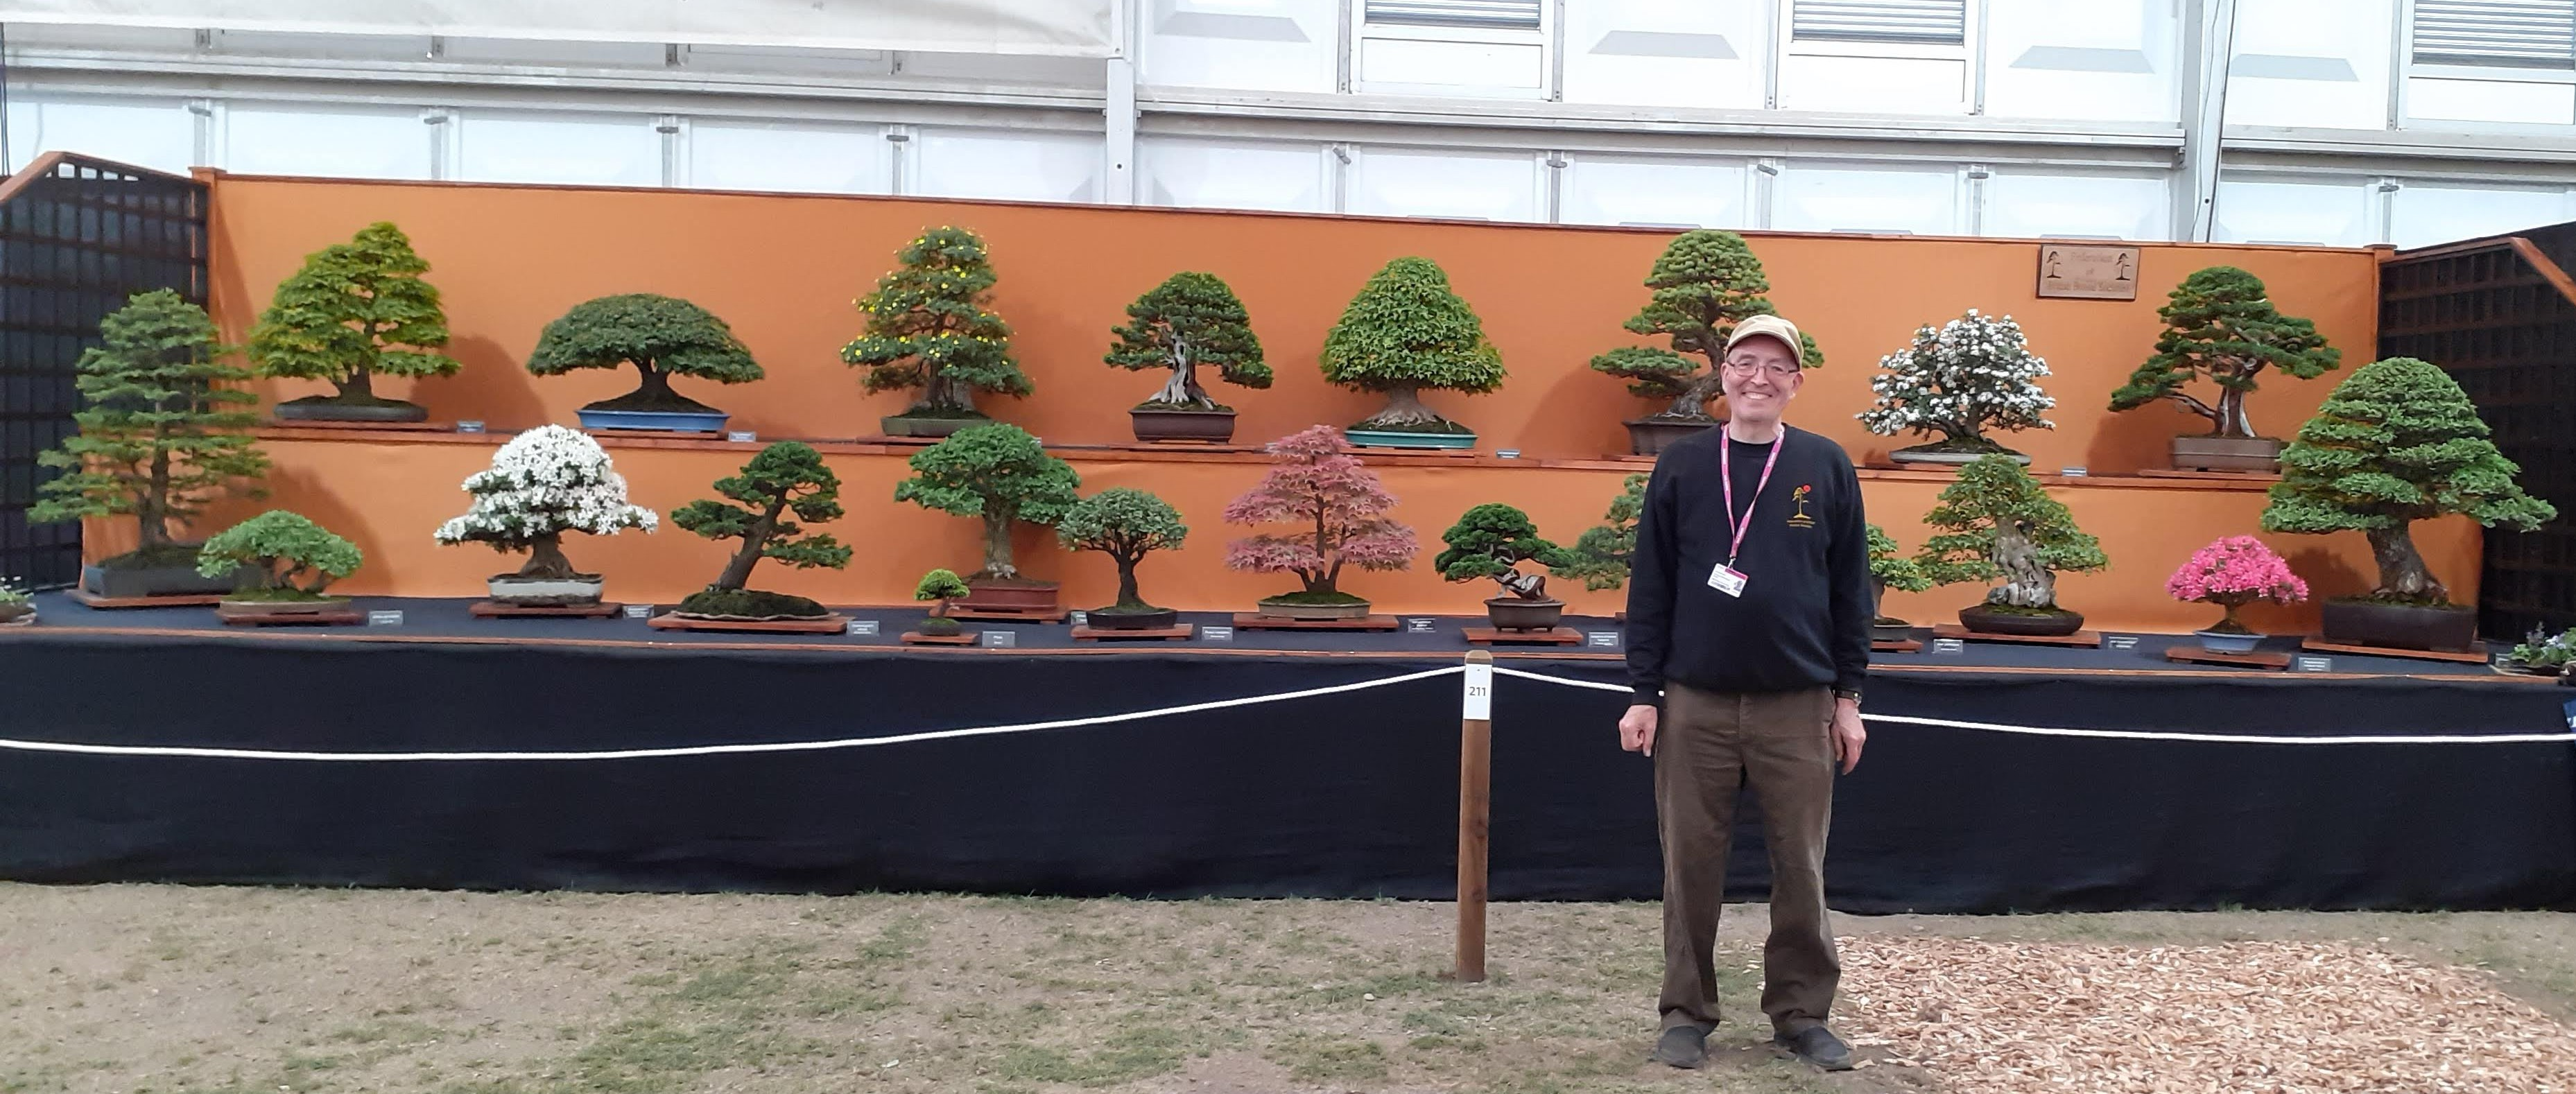
\includegraphics[width=1.0\textwidth]{2025_01/res/chris_durne.jpg}
    \centerline{\emph{Chris standing in front of the gold medal Bonsai display he curated at the Chelsea Flower Show.}}
\end{figure*}

\headline{{\textbf{\Large\sffamily Bonsai Roots:}}\\
          {\textbf{\large\sffamily Meet the Members of TWBC}}}
\label{2025-01-roots}
\noindent
Welcome to the latest edition of \emph{Bonsai Roots}, our monthly column where we highlight the individuals who make up the heart of the Twickenham Bonsai Club.
This feature aims to deepen connections within our community and provide potential new members with a closer look at the people who shape our vibrant club.
This month, we're pleased to introduce \textbf{Chris Durne}, a passionate bonsai enthusiast who recently joined us.
Many of you may remember Chris from November last year when he shared his insights on the \emph{selection and judging criteria} at the prestigious \textbf{Chelsea Flower Show}.
With over 30 years of experience in bonsai and a wealth of knowledge to offer, we're excited to learn more about Chris and his bonsai journey.

\begin{itemize}
    \item \textbf{What's your name and where in the country do you live?}

    \emph{My name is Chris Durne, and I live in Wandsworth, South West London.}

    \item \textbf{What are your favourite species of tree and why?}

    \emph{My favourite species include the English Elm, Scots Pine, and Chinese Elm. The English Elm is a favourite native species, while the Scots Pine is highly adaptable and can be shaped when dormant. The Chinese Elm is incredibly versatile, thriving as both a Mame and a larger tree, and is tolerant of neglect, especially when grown indoors.}

    \item \textbf{What aspect of bonsai do you enjoy?}

    \emph{I enjoy developing my bonsai over many years. There's something very satisfying about knowing the right techniques to use and when, in order to keep the tree healthy. It's a real horticultural challenge, and gaining species-specific knowledge over time has kept my interest alive.}

    \item \textbf{What aspects of bonsai do you find most challenging?}

    \emph{Wiring a complete tree to define the pads is something I really enjoy, but cutting off all the wire once the design has set is challenging. Scots Pines, in particular, require constant wiring to maintain their profile.}

    \item \textbf{Who or what inspires you throughout your bonsai journey?}

    \emph{I've been inspired by the talented members of Bonsai Kai, especially people like Ken Norman, Kevin Willson, Lee Verhorevoort, and Corin Tomlinson, who led demonstrations. Peter Shields, who was the Secretary of Bonsai Kai, taught me many growing techniques and played a big role in my development as a bonsai enthusiast.}

    \item \textbf{How long have you been interested in keeping bonsai?}

    \emph{I've been interested in bonsai since 1985, so I've been involved in the hobby for over 30 years now.}

    \item \textbf{What stimulated your interest in bonsai?}

    \emph{My interest in bonsai was first sparked when I saw some miniature trees in my neighbour's garden. I learned that these trees were bonsai, and I was intrigued. My neighbour encouraged me to attend a society in Central London, and from there, my passion for bonsai grew.}

    \item \textbf{If you could give someone new to bonsai any tips, what would it be?}

    \emph{My biggest tip would be to avoid styling or working on a tree in the same season that you dig it up. It's too stressful for the tree. I recommend allowing the tree to recover for a year in the proper substrate before doing any work on it. I also advise alternating between root work and structural styling to keep the tree healthy.}

    \item \textbf{Why do you enjoy being part of TWBC, and do you have any ideas or suggestions for the club's future?}

    \emph{TW is very welcoming to everyone who wishes to learn, and the communication between members is truly inspiring.}

    \item \textbf{One word to describe what bonsai means to you?}

    \emph{Peace and Calm. (Ok, two words!)}

    \item \textbf{What are your future goals regarding your own trees and learning more about the hobby?}

    \emph{After living in the USA for four years, I sold most of my noteworthy trees to fund the airline tickets! I'm now rebuilding my collection by working on a garden full of material I plan to transform. I even have some plants waiting their turn to be styled that are 50 years old.}

    \item \textbf{How would you like to see your bonsai journey progress in the future?}

    \emph{I hope to continue developing and refining bonsai over the years. In the future, I'd like to continue contributing to exhibits at the Chelsea Flower Show and helping the Federation of British Bonsai Societies earn more gold medals as I did in the past. Most importantly, I want to keep sharing my passion and knowledge with others in the bonsai community.}

\end{itemize}

We hope you've enjoyed learning more about Chris's inspiring bonsai journey.
Stay tuned to \emph{Bonsai Roots} for more member stories in the coming months!
\closearticle

\vfill
\begin{center}
	\includegraphics[width=0.95\columnwidth]{res/filler_c.png}
\end{center}
\columnbreak
